\begin{figure}[h!]
\centering
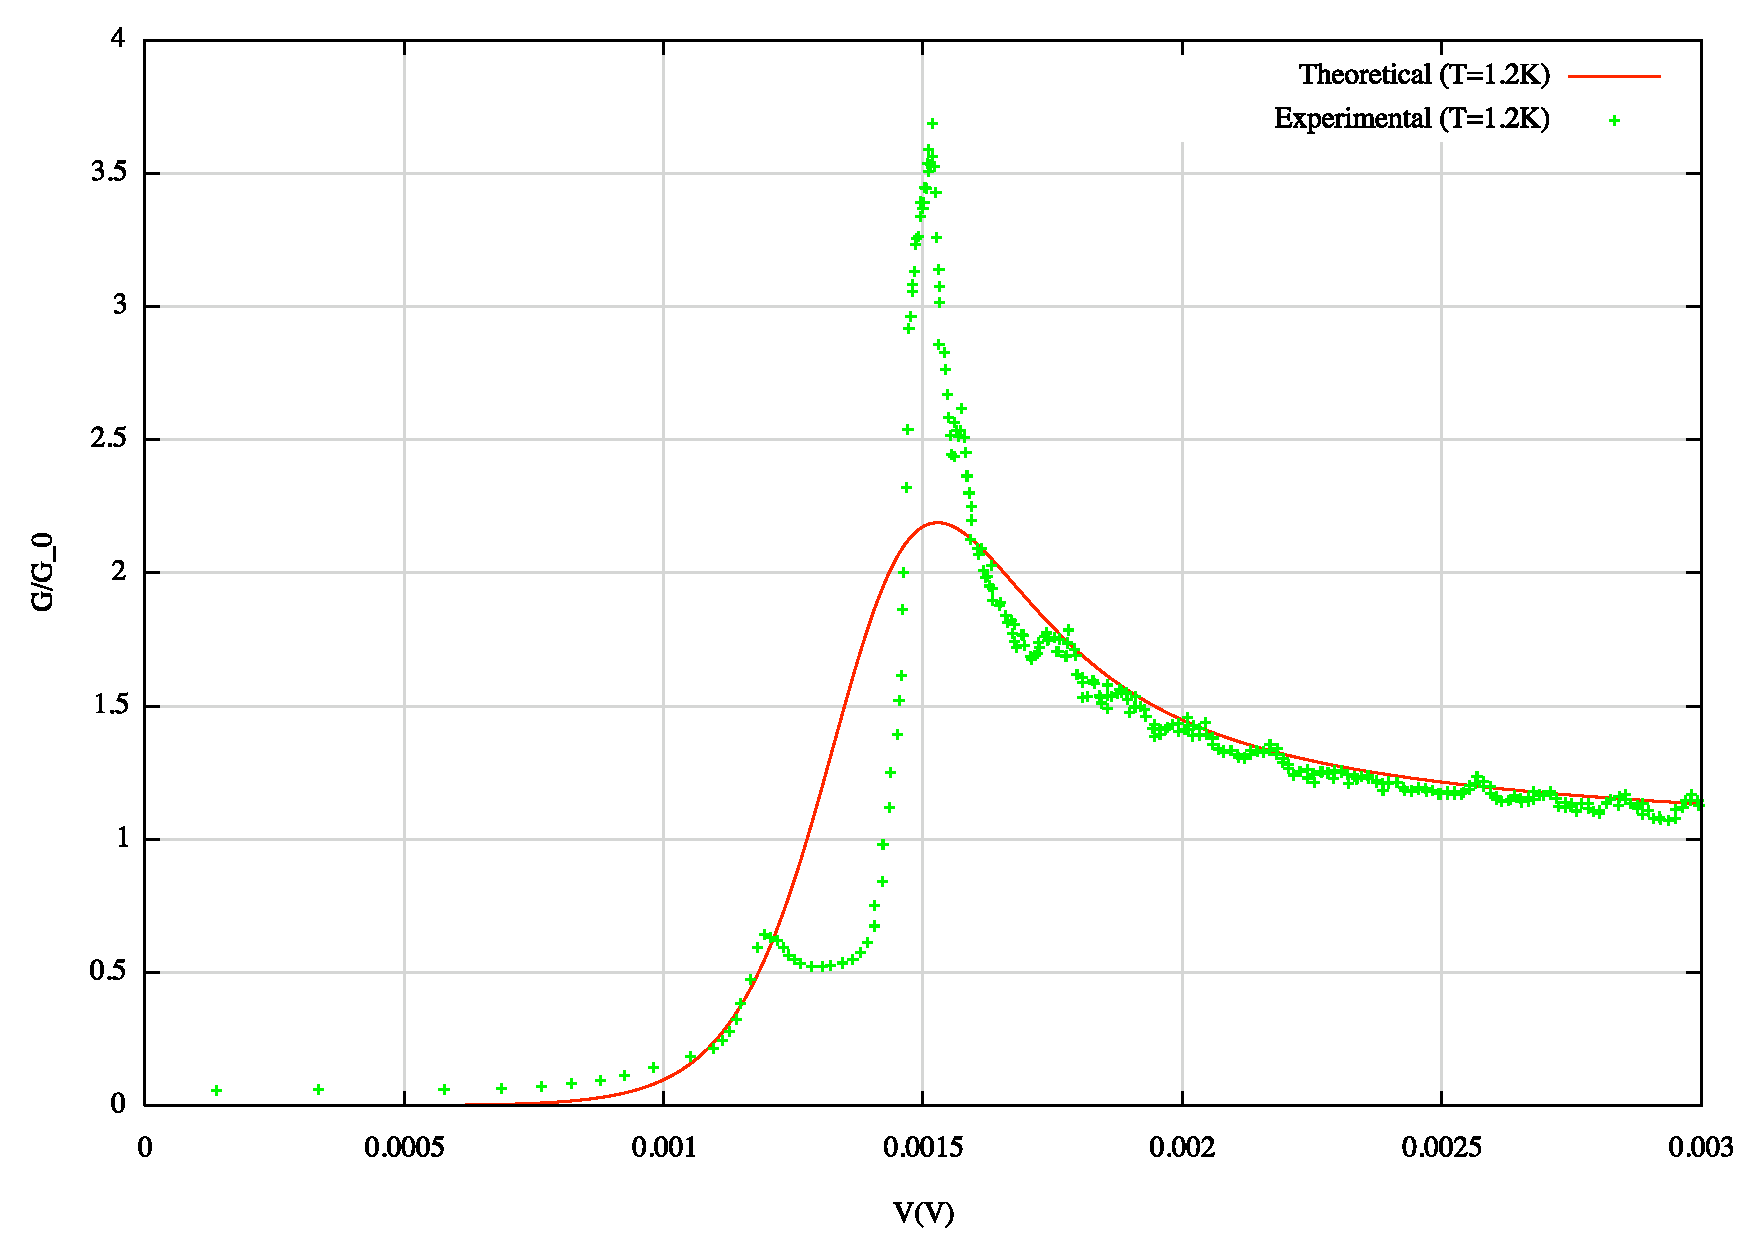
\includegraphics[width=0.45\textwidth]{gv_theo_exp_10}
\caption{\small Experimental data and BCS theoretical prediction for $1.2 K$. There is a second peak due to the superconductor transition of some parts of the Aluminum.
\label{gv_theo_exp_10}}
\end{figure}

The measurement at the lowest temperature that we could perform gives qualitatively different results. In fig. \ref{gv_theo_exp_10} can be seen the appearance of new effects. The transition temperature $T_c$ for Aluminum is $1.140 K$, and we have established experimentally the temperature for data as $1.2 K$. However, due to the difference between bulk properties and those that we must consider here for thin films, the $T_c$ is a little bit greater (see \cite{films},).

The situation is qualitatively clear now, i.e. the temperature has fallen enough to let some portions of Aluminum change to superconducting state, creating this combined effect between normal-superconductor and superconductor-superconductor junctions. It can be explained by considering a sum of junctions of these two kinds in parallel, so as to produce an I-V curve with peaks inside the gap of the Aluminum. For a superconductor-superconductor junction appear two peaks, located at $| \Delta_1-\Delta_2|$ and $(\Delta_1+\Delta_2)$.

